\subsection{Mismatched Crowdsourcing}
\label{sec:methodsmc}

Mismatched transcriptions were collected from crowd workers (Turkers)
on Amazon Mechanical Turk~\cite{MTurk} for all the data listed in
Table~\ref{tab:data}.  The crowdsourcing task setup is described
in~\cite{JHJ15b}.  Each 5-sec speech segment was further split into 4
non-overlapping segments to make the non-native listening task
easier. The crowdsourcing task was set up as described
in~\cite{JHJ15b}; briefly, the short segments were played to Turkers,
who transcribed what they heard (typically in the form of nonsense
syllables) using English orthography. Each short recording segment was
transcribed by 10 distinct Turkers. More than 2500 Turkers
participated in these tasks, with roughly 30\% of them claiming to
know only English. (Spanish, French, German, Japanese, Chinese were
some of the other languages listed by the Turkers.)

\begin{table}[t]
\centering
\begin{tabular}{|c||c|c|c|c|c|c|c|}
  \hline
  & \multicolumn{7}{|c|}{Language (ISO 639-3 Code)}\\ \hline
& arb & yue & nld & hun & cmn & swh & urd \\ \hline\hline
Dev set (1-best PER) & 65.8 & 66.4 & 68.9 & 63.7 & 70.9 & 47.6 & 67.2 \\
Eval set (1-best PER) & 66.2 & 67.8 & 70.9 & 63.5 & 69.6 & 50.3 & 70.5 \\\hline
\end{tabular}
\caption{Error rates (PER) of probabilistic transcripts computed from
  mismatched crowdsourcing (non-native human listeners): Phone error
  rate (PER) of the 1-best path through the probabilistic
  transcription, $\phi^*=\argmax\rho(\phi|T)$, development and
  evaluation sets.}
\label{tab:LPER}
\end{table}

A crude measure of the quality of the PTs is given by the phone error
rate between $\phi^* = \argmax_{\phi} \rho(\phi|T)$ and the reference
phone sequences. Table~\ref{tab:LPER} lists these 1-best error rates
on the SBS development and evaluation sets, for all seven
languages. However, the 1-best error rates do not accurately reflect
the extent of information in the PTs that can be leveraged during ASR
adaptation.  Consider, for example, the four Hindi
phones~\ipa{[p,p\textsuperscript{h},b,\"*b]}.  An attentive
English-speaking transcriber must choose between the two letters
$<$p,b$>$ in order to represent any of these four phones.  The
misperception G2P therefore maps the letters $<$p,b$>$ into a
distribution over the phones~\ipa{[p,p\textsuperscript{h},b,\"*b]}.
There is no reason to expect that the maximizer of
$\rho(\phi|\lambda)$ is correct, but there is good reason to expect
the correct answer to be a member of a short $N$-best list ($N\le 4$
phones/grapheme).  A fuller picture is therefore obtained by
considering a collection of sequences $\phi$ that are almost as
probable as $\phi^*$ according to our model. Figure~\ref{fig:listPER}
shows the trend of phone error rates (for three languages) obtained by
using collections $\phi$ of increasing size, plotted against an
entropy estimate of $\phi$, e.g., 1 bit of entropy allows two equally
probable choices for each phone in $\phi$. We note that the phone
error rates significantly drop across all languages, staying within 1
bit of entropy per phone, illustrating the extent of information
captured by the PTs.

\begin{figure}[t!]
\begin{center}
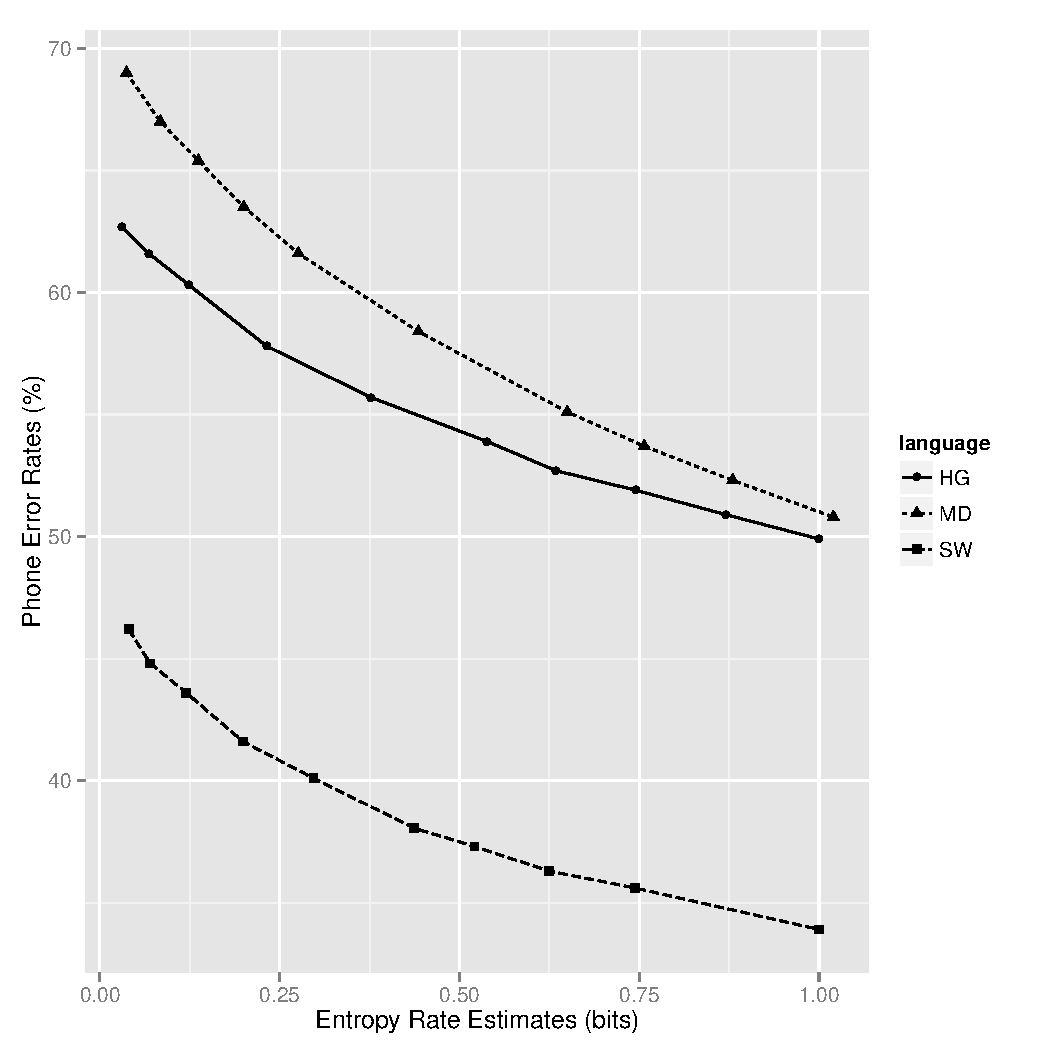
\includegraphics[width=4in]{../figs/listper.pdf}
\end{center}
\caption{Phone error rates plotted against entropy rate estimates of phone sequences in three different languages.}
\label{fig:listPER}
\end{figure}
